% !TeX spellcheck = en

\chapter{Fundamentals}
\label{sec:theorie}
This chapter introduces theoretical background of the presented research problem. First, the concept of mixed reality (MR) followed by an introduction of six degree of freedom (6-DoF) environment and the difference to the three degree of freedom (3-DoF) are described. The term motion-to-photon latency (M2P) is covered, followed by a short discussion about an influence of M2P latency on the decreasing of user experience. The new developed cloud-based rendering and streaming approach is shortly discussed in this chapter. The last section of this chapter highlights challenges with the prediction of viewer's head pose that arises in modern XR applications in connection especially with the added network latency due the using of remote cloud server for computational offload. The section \ref{sec:related} overviews the existing works done in the research field using traditional algorithms and recurrent neural networks. 
%##############################################
\section{Mixed reality with HMD}
\label{sec:theorie:ar}
Mixed reality makes possible to break down the border between the virtual and real world and provides today an experience that just a short-time ago we could only imagine when watching the sci-fi movies. Terms Virtual Reality (VR), Augmented reality (AR) and Mixed reality (MR) are often used interchangeably. VR creates the virtual environment around user and tricks human's senses into thinking one is in a different environment. AR adds a virtual object to the real world that we can see through the lenses of special developed Head Mounted Display (HMD). Thus realistic images, sounds, and other sensations can be generated by a powerful HMD and projected on transparent holographic lenses giving a user the feeling that virtual objects have size and density. However, AR does not allow interactions between users and the virtual objects added to the real-world scene. MR combines the advantages of the VR and AR and adds an interaction between real and artificial elements. Thus users can directly interact with virtual objects (with operations such as scaling, rotation, or translation) in the real environment using their hands. For example, in MR Application virtual objects can be placed on the real table in the user's room, picked up with a hand and moved to another place.\\
%##############################################
Volumetric video (VV) is a new content creation approach to be used within AR and MR applications \cite{user_behav_volumetric}. Volumetric video allows to view recorded information from a range of different angles, as if an observer was physically presented in the room when video was captured by cameras and could move around the object. This thesis uses volumetric video object placed in the real environment when running developed MR Application for collection the user's position and rotation data. Refer sections \ref{sec:theorie:cloud} and \ref{sec:impl:model:dev:unity} for more details about VV and how it was used in thesis. 
%############################################
\begin{wrapfigure}{L}{0.5\textwidth}
	\centering
	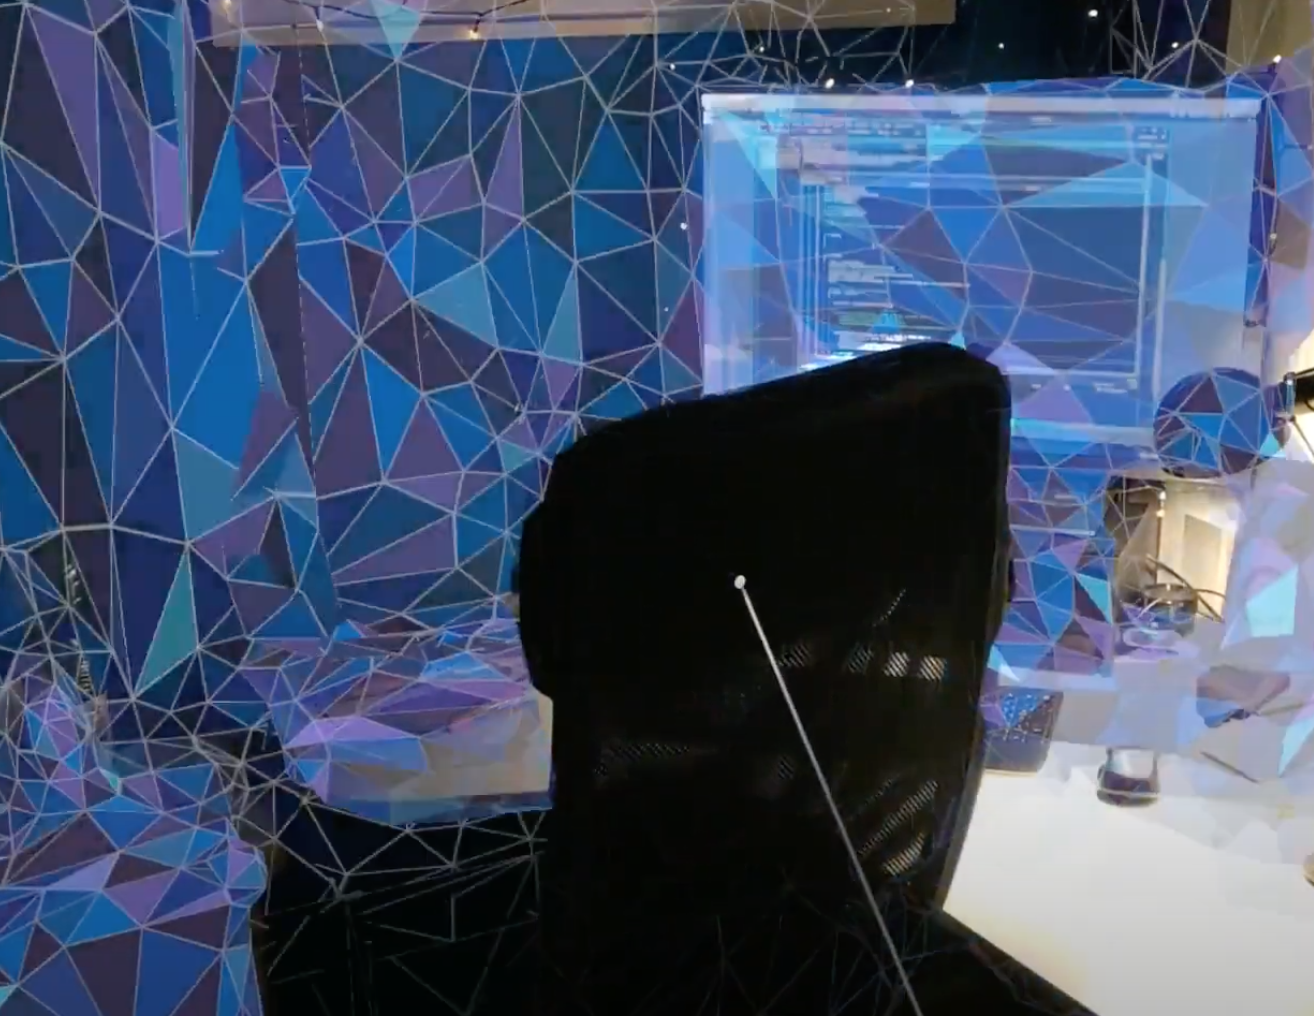
\includegraphics[width=0.47\textwidth]{gfx/hololens_env.png}
	\caption{\label{fig:holo2_env}HoloLens 2 maps itself with a mesh.}
\end{wrapfigure}

Nowadays different HMD with varying performance levels and prices are available on the market. In this thesis, Microsoft HoloLens 2 was used for MR experience and data collection. It is an updated version of the previous generation HoloLens 1 headset from Microsoft with such improved feature as display resolution, field of view, weight, battery lifetime. By using the AHAT (Articulated HAnd Tracking) depth camera, the HoloLens 2 can capture hand movements to obtain hand tracking data. The build-in tracking systems allows HoloLens to understand the environment around the user and to place stable and accurate holograms on the correct places where they intended to be by the developer of MR Application. The data used to track users is represented in the spatial map\footcite{https://docs.microsoft.com/en-us/hololens/hololens-environment-considerations}. When VR Application is starting on HoloLens, HoloLens uses unique environmental landmarks to locate itself in a space. The mesh graphic spreading over the space is seen, as illustrated in Fig.  \ref{fig:holo2_env}, during the Application launch and this means a device is mapping to surroundings. As user moves with HMD on their head, built-in cameras continuously scan the environment and construct virtual world geometry for real-world objects. The primary stereo rendering component attached to HMD can be accessed from Unity and thus the position and orientation can obtained for thesis purposes. 

%##############################################
\section{Six degrees of freedom}
\label{sec:theorie:6dof} 
Term \textit{degrees of freedom} describes how users interact with a virtual environment and how they can move inside it. Within 3-DoF space user has only three possibilities: look left and right, look up and down and pivot left and right. 3-DoF space does not allow to move throughout the virtual space. Thus only rotational movement can be tracked. In 3-DoF VR Application multimedia content is the omnidirectional or spherical video, which represents an entire 360$^{\circ}$ environment on a virtual sphere \cite{6-dof_metrics}. In 3-DoF space HMD enables to display only a portion of the environment around a user. User is virtually positioned at the centre of a sphere as shown in Fig. \ref{fig:3-6dof}, media is displayed from an inward position and user can only change the viewing direction (i.e., by looking up/down or left/right or tilting the head side to side) \cite{6-dof_metrics} but can not interact with a media by moving closer/further. Wherever user moves with a HMD on their head, they will remain placed in the  at the centre of a sphere and distance to a content can not be changed. 
\begin{wrapfigure}{R}{0.4\textwidth}
	\centering
	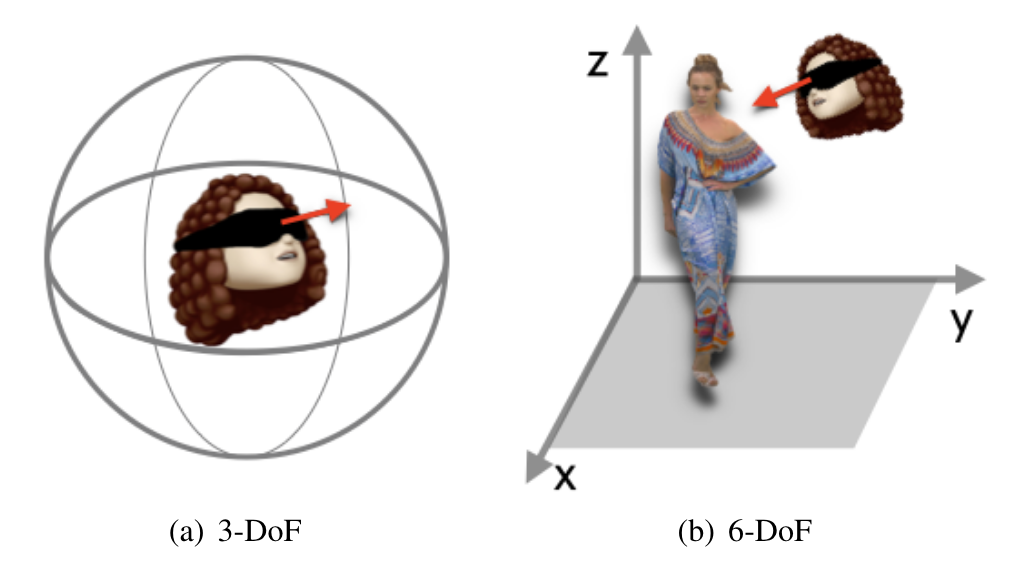
\includegraphics[width=0.37\textwidth]{gfx/3-6dof.png}
	\caption{\label{fig:3-6dof}Viewing paradigm in 3- and 6-DoF VR. Source: \cite{6-dof_metrics}}
\end{wrapfigure}


\section{Motion-to-photon latency}
\label{sec:theorie:m2p}

\section{Cloud-based volumetric video streaming}
\label{sec:theorie:cloud}
% User Behaviour Analysis of Volumetric Video in Augmented Reality

\section{Challenges of head motion prediction}
\label{sec:theorie:head_pred}
All modern HMD has a position tracker, a device or a system of devices, that is responsible for reporting  the position and orientation of HMD to the computational unit that generates the virtual environment images displayed in the HMD. These images represent the view that a wearer of HMD would have seen if user was present in VR at the position and orientation reported by position tracker \cite{hmd}.\\
While the task of position tracking is performed by HMD hardware, the task of position prediction of the movement of human body in the virtual reality remains challenging, and it is still complicate to achieve high-precision estimation. Recurrent neural networks have recently shown promising results in many machine learning tasks, especially when input and/or output are of variable length and are coming as time series with a sequential order.  Unfortunately, the known problem of RNN that was observed many years ago by e.g., \textit{Bengio et al., 1994} that it is difficult to train RNNs to capture long-term dependencies because the gradients tend to either vanish (most of the time) or explode (rarely, but with severe effects) \cite{rnn_difficults}. New approaches are needed to be implemented to reduce the negative impacts of this issue. Since traditional recurrent unit overwrites its content at each time-step, a LSTM unit is able to decide whether to keep the existing memory via the introduced gates. The Long Short-Term Memory (LSTM) has a number of minor modifications \cite{empirical_evaluation} since it was initially proposed in work \cite{lstm_orig}. Another approach called a gated recurrent unit (GRU) can adaptively capture dependencies of different time scales without having a separate memory cells \cite{empirical_evaluation}. These two approaches can help to find the long-term dependencies in the data obtained from HMD that are otherwise are hidden by the effect of short-term dependencies from the standard RNN models.\\
%============================================
Not only the NN architecture is important for high prediction accuracy. Understanding how users interact and behave in AR or VR is a key for preparing the correct dataset when working with HMD's sensors. The experiment done by \textit{Zerman et al., 2021} found out that users preferred to stay in front of static point clouds and 1-1.5 meter away from them and spent more time looking at the frontal view and faces of human models \cite{user_behav_volumetric}. The navigation trajectories of users within a 6-Degrees-of-Freedom (DoF) should be additionally investigated. An extra level of interaction between user and content is available in 6-DoF environment. The user has now the freedom to change the viewing direction (rotating and translating the head as in 3DoF) but also to change position inside the VR environment \cite{new_challenge}. In a 3-DoF environment, users are viewing a portion of the omnidirectional content all the time being positioned at the centre of the spherical content. Thus it is important to understand that a distance between user and content is constant during the interaction \cite{new_challenge}. In a 6-DoF, however, the distance changes over time when user moves due to the added degrees of freedom. Thus viewport’s center position is not sufficient for tracking the trajectories, the additional metrics such the spatial coordinates and user orientation are needed to obtain the point of origin. Following \cite{new_challenge} \textit{Rossi et al, 2021} authored same year another work \cite{6-dof_metrics} dedicated 6-DoF metrics. Researchers proposed to change the video detailing based on user distance to the volumetric object. The closer users are to the volumetric content, the smaller and more detailed is the portion of the displayed content; the farther they are, the bigger but with fewer details becomes the displayed portion \cite{6-dof_metrics}. \textit{Rossi et al, 2021} experimented with different metrics to perform clustering in order to detect group of users with similar behavior in VR. The most promising metric seems to be based on the user position on the virtual floor. Metrics based only on viewport center and distance failed in detecting the group of users, which in the ground-truth case form their own cluster, as similar and divided them instead in different clusters \cite{6-dof_metrics}. For the trajectory detection best performed a metrics based on user position on the virtual floor, distance and viewport center. Thus not only the way in which users interact within a 3- and 6-DoF environment is fundamentally different. New physical settings and locomotion functionalities given to users also prevent a straightforward extension of current 3-DoF algorithms to 6-DoF \cite{6-dof_metrics}. The analysis above leads to the conclusions that prediction of the user's position and orientation on 6-DoF not only a contemporary but also a challenging task that requires new metrics and approaches to be investigated and implemented. 